% !TEX program = xelatex
% Compile with:  xelatex -shell-escape Rules.tex   (needed by the svg package)
\documentclass[10pt,a4paper]{article}
\usepackage[margin=2cm]{geometry}
\usepackage[skip=4pt]{parskip}
\usepackage{enumitem}
\usepackage{amssymb}
\usepackage{fontspec}
\usepackage{svg}            % converts .svg via Inkscape at compile time
% \svgpath{{figures/}}      % uncomment if the SVGs live in a figures/ subfolder

\newfontfamily\gujaratifont{Noto Serif Gujarati}[Script=Gujarati]
\newcommand{\guj}[1]{{\gujaratifont #1}}

\newcommand{\ruletitle}[2]{\subsection*{Rule #1 --- #2}}

\title{\textbf{Kauda Baji: Proposed Rules}\\[2mm]
\large For review}
\author{M. Naik}
\date{July 2026}

\begin{document}
\maketitle

\section*{Why this document}

I'm currently working on a hobby project to build an AI agent that plays Kauda Baji.
The idea is to build a complete model of the game in code, then design AI agents that can play it.
In the future, time permitting, there may even be a robot that plays the game with you in real life.

I've progressed though making models for the board, player, pieces, and moves.
The next remaining step is defining the rules.

And this is where I need your help!

The ask is for you to please read this document and provide feedback if you agree or disagree with each rule.
Because a computer will be playing using these rules, they must be fully unambiguous.
Anything marked as a \emph{question for the family} at the end is genuinely open --- I want your
opinion.

If the rule set is agreed upon by all parties, it will enable my project progress.

I would be grateful for your time and feedback.

\section*{Terms used}

Our game is played in Gujarati, but code is typically written in English so I've had to come up with some terms for common concepts.
Here are the terms I will use in this document, and their meanings and translations.

\begin{description}[leftmargin=2em, style=nextline]

  \item[Piece] Trans.(\guj{કૂકી}, \guj{કૂકડી}) - One of 6 movable objects belonging to one player.

  \item[Tuple] Trans.(\guj{દૂગલું}, \guj{તિગલું}, \guj{ચૌગલું}, ...) - A player's own pieces stacked on the same square
    and moving together as a unit.

  \item[Tuple Size] The number of pieces in a tuple. A \guj{દૂગલું} has size 2, a \guj{ચૌગલું} has size 4, etc.

  \item[Kaudi] One of six cowrie shells thrown together to generate a move.
    Plural: \emph{kaudis}.

  \item[Safe square] A square marked with a corner-to-corner cross. The
    starting squares and the centre square are safe.

  \item[Kill] Removing an opponent's tuple from the board. Killed pieces go
    back to their owner's starting square and begin their journey again.

\end{description}

\section*{The board and pieces}

\begin{center}
\begin{minipage}{0.45\textwidth}
  \centering
  \includesvg[width=0.85\textwidth]{figures/kauda_baji_board}
\end{minipage}%
\hspace{0.02\textwidth}
\begin{minipage}{0.45\textwidth}
  \centering
  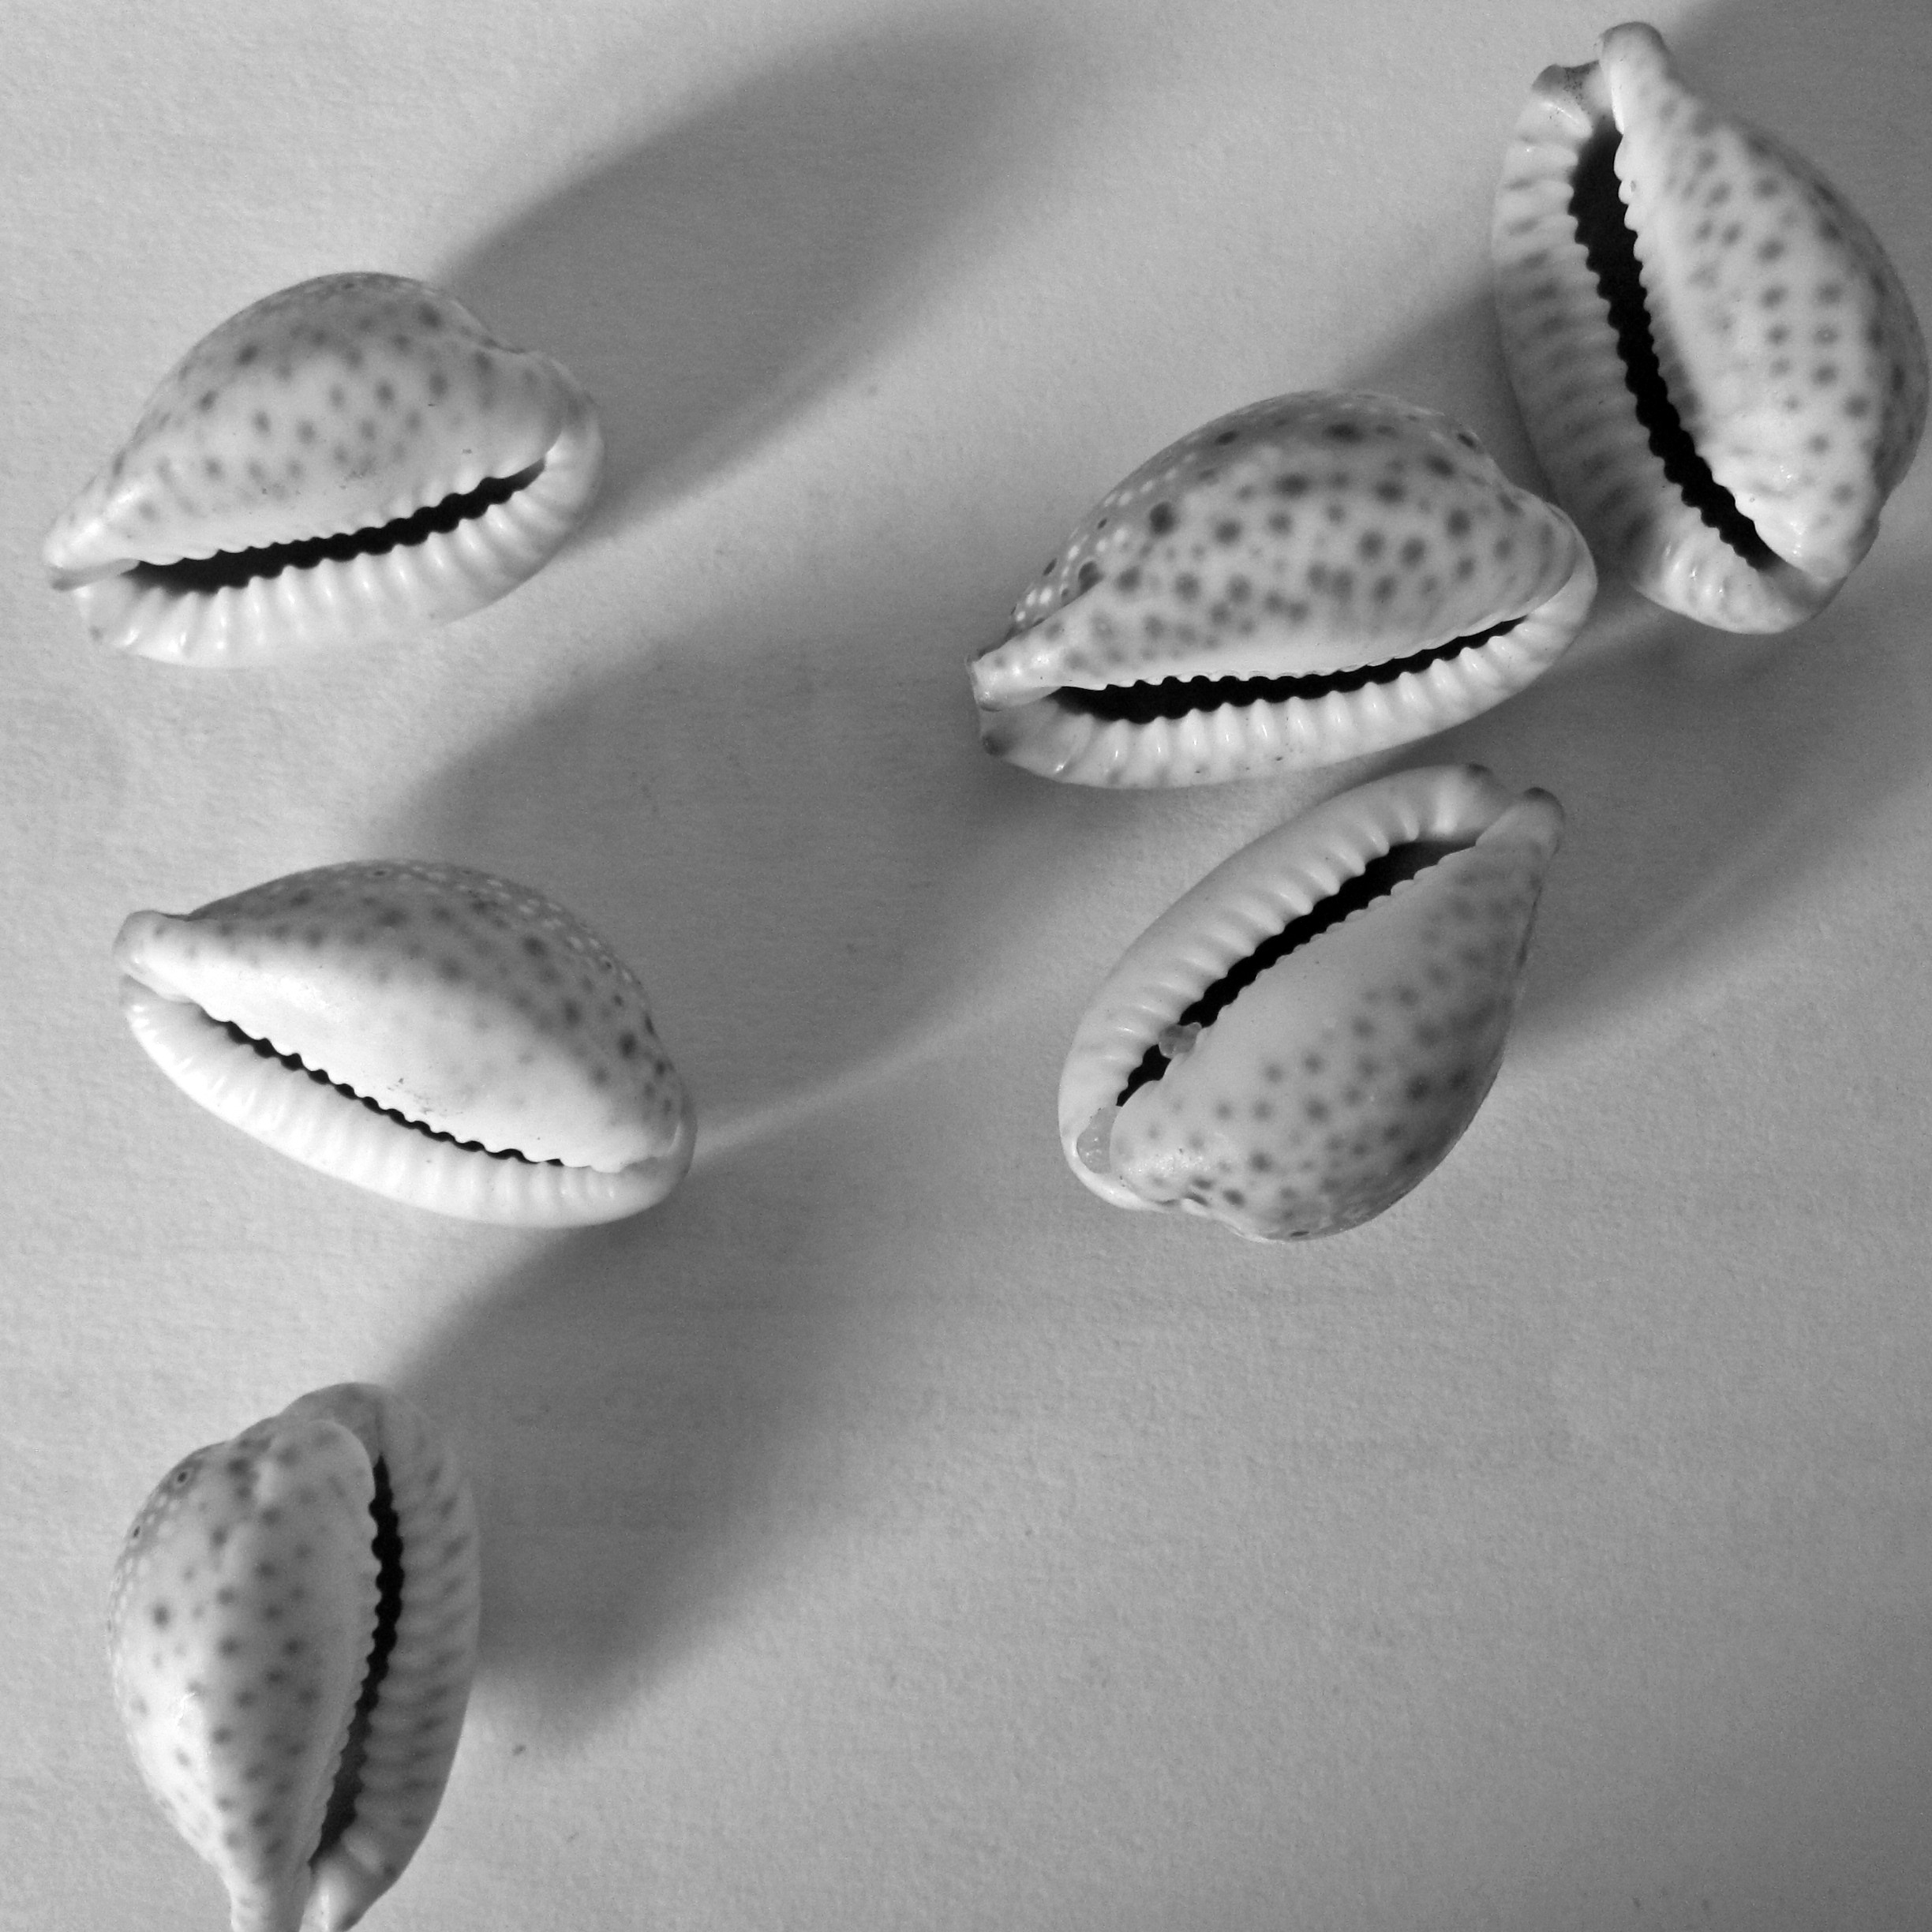
\includegraphics[width=0.85\textwidth]{figures/kaudi_shells_bw.jpg}
\end{minipage}
\end{center}

The board is a 7$\times$7 grid of squares. Four players sit at the four edges;
each player owns the edge nearest them.

Each player has six pieces of their own colour. 
Every player's pieces start on the same square: the crossed square in the
middle of that player's own edge. This is the player's \textbf{starting
square}. From there, pieces travel around and inward, and all four players
finish on the single square at the very centre of the board.

Twelve squares carry a corner-to-corner cross, and one more sits at the centre
--- these are the \textbf{safe squares}, marked in the diagram above. Every
other square is ordinary. What makes safe squares special is covered in the
rules below.

Moves are generated by throwing a set of six \emph{kaudis} --- cowrie shells
--- together. Each kaudi can land one of two ways: mouth-up or mouth-down.
How a throw translates into a move is covered in a later rules section.

\begin{center}
\begin{minipage}{0.45\textwidth}
  \centering
  \includesvg[width=0.85\textwidth]{figures/kauda_baji_path}
\end{minipage}%
\end{center}


Every piece follows the same route from its starting square to the centre. The
route is identical for all four players, just rotated to begin at each player's
own edge.

A piece begins on its \textbf{starting square} --- the crossed square in the
middle of the player's edge --- and travels anticlockwise around the outer
ring of the board. At the \textbf{first arrow}, it turns inward onto the
first inner band and continues \textbf{clockwise} around that band. At the
\textbf{second arrow}, it turns inward again onto the second inner band,
still travelling clockwise. The \textbf{third and final arrow} then carries
the piece onto the centre square, completing its journey.

The objective of the game is to get all six pieces from the starting square to the centre square. The first player to do so wins.


\section*{The rules}

% Kaudi throw outcomes are based on the number of kaudis that end up mouth-up after the throw.
% If no kaudis land mouth-up, the player gets an outcome of 12 squares.
% Thus the possible outcomes of a throw are 1, 2, 3, 4, 5, 6 or 12 squares.
% Svgs of 5, 6, and 12 kaudis mouth-up outcomes.

% Before the game begins, a round of kaudi throws is made to determine the first player.
% First turn is given to the player that rolls the highest value on the kaudis
% Turns are Anticlockwise from there. 

% A turn begins with a throw of the kaudis. 
% Throwing an outcome of 6 or 12 allows the player to throw again while banking the prior value. 
% However, if a player throws 6 or 12 three times in a row, they forfeit their turn.

% The outcome of the throw(s) is then  used to move pieces around the board.
% The player may move any one of their pieces by an equal number of squares. 

% Multiple throw outcomes (e.g. 6 and 3) can be used to move a single or multiple pieces, in any combination.
% However, individual throw values cannot be split between peices.
% Example SVG

% Going around rules -  At each of these three arrows, the player may choose to follow the arrow and turn inward,  
% or continue straight and stay on the current band for strategig reasons. 

% Single Piece Kill Rules
% Kills give additional throws.
% Example SVGs

% Safe Squares kill avoidance rule

% Markut rule

% Tuple Forming (coexistance and then movement together)
% Example SVGs

% Assignment of throws to tuples (divide rule)
% Example SVG

% Tuple Dissolving (from safe squares only)

% Kill Rules Generalised to Tuples
% Enter Rules
% Exit Rules
% Also gives a single bonus throw.
% Played out Pattern Examples


\ruletitle{1}{Landing on an opponent: equal or bigger kills}

If your tuple lands on a square holding an opponent's tuple, and your tuple is
the \textbf{same size or bigger}, the opponent's tuple is killed. Your tuple
takes the square; their pieces go back to their start.

% FIGURE: rule 1 -- before/after: Red 2 lands on Blue 2, Blue killed
% \begin{center}
%   \includesvg[width=0.75\textwidth]{rule1_landing_kill}
% \end{center}

The same happens if the landing tuple is strictly bigger --- a Red~3 landing
on a Blue~2 kills it just the same. Equal size is enough; the attacker never
needs to outnumber the defender.

\ruletitle{2}{Landing on an opponent: smaller coexists}

If your tuple lands on a square holding an opponent's tuple and yours is
\textbf{strictly smaller}, nothing is killed. Both tuples share the square.

% FIGURE: rule 2 -- before/after: Red 1 lands on Blue 2, both share the square
% \begin{center}
%   \includesvg[width=0.75\textwidth]{rule2_coexist}
% \end{center}

Notice what this means: whenever two opponents share a square, the tuple that
was there first is always the bigger one. The smaller tuple is a guest on a
stronger tuple's square.

\ruletitle{3}{Leaving a shared square: the bigger tuple kills on exit}

When two opponents share a square and the \textbf{strictly bigger} tuple moves
away, it kills the smaller tuple as it leaves.

% FIGURE: rule 3a -- before/after: Blue 3 departs shared square, Red 1 killed
% \begin{center}
%   \includesvg[width=0.75\textwidth]{rule3a_exit_kill}
% \end{center}

The reverse is free: if the \emph{smaller} tuple moves away first, no kill
happens --- it simply escapes.

% FIGURE: rule 3b -- before/after: Red 1 departs shared square, no kill
% \begin{center}
%   \includesvg[width=0.75\textwidth]{rule3b_escape}
% \end{center}

So sharing a square is dangerous for the guest. The smaller tuple sits under
threat until either it leaves, or the bigger tuple leaves and kills it on the
way out.

\ruletitle{4}{Safe squares: no kills, ever}

No kill of any kind can happen on a safe square. Any number of tuples, of any
sizes, from any players, can share a safe square. Landing there kills nothing,
and leaving a shared safe square kills nothing.

% FIGURE: rule 4 -- before/after: Red 3 lands on Blue 2 on a safe square, no kill
% \begin{center}
%   \includesvg[width=0.75\textwidth]{rule4_safe_square}
% \end{center}

\ruletitle{5}{Three or more players on one square: settle each pair separately}

When a tuple lands on a square holding tuples from more than one opponent,
apply Rules 1 and 2 to \textbf{each opponent separately}. The lander kills
every opponent tuple that is its size or smaller, and coexists with every
opponent tuple that is bigger.

% FIGURE: rule 5 -- before/after: Red 2 lands on square with Green 1 and Blue 3;
% Green 1 killed (Red 2 >= Green 1), Blue 3 survives (Red 2 < Blue 3)
% \begin{center}
%   \includesvg[width=0.75\textwidth]{rule5_pairwise}
% \end{center}

Exit kills work the same way: a departing tuple kills every strictly smaller
opponent tuple it leaves behind, and spares the rest.

\section*{What follows from these rules}

These are not extra rules --- they are consequences of Rules 1--5. I list them
because they answer situations that caused arguments in the past.

\begin{itemize}[leftmargin=2em]
  \item \textbf{Two opponent tuples of equal size can never share an ordinary
    square.} Landing with equal size kills (Rule 1), so the situation can
    never arise in the first place.
  \item \textbf{On a shared ordinary square, the resident is always bigger
    than the guest.} Coexistence only ever begins with a smaller tuple landing
    on a bigger one (Rule 2).
  \item \textbf{Big tuples are strong but slow to threaten.} A size-3 tuple
    can only be killed by a size-3 or bigger landing on it --- but it also
    spends three pieces on one square.
  \item \textbf{A lone piece is never safe on an opponent's square.} As a
    guest it can be killed the moment the resident moves (Rule 3).
\end{itemize}

\section*{Questions for the family}

\begin{enumerate}[leftmargin=2em]
  \item \textbf{Does a kill earn an extra throw of the kaudis?} Some of us
    remember playing with this, some without.
  \item \textbf{Must a player make at least one kill before their pieces may
    enter the inner rings?} Several Chowka Bhara variants play this way. Do
    we?
  \item \textbf{When killed pieces return to the start, do they return as
    single pieces, or as the tuple they were?} My proposal: as single pieces
    --- the tuple is destroyed, not relocated.
\end{enumerate}

Please mark up anything you disagree with, or reply with the version you
remember. Once we agree, this becomes the reference for both the physical
board and the computer version I am building.

{\small\emph{Kaudi photo: Sodabottle, CC BY-SA 3.0, via Wikimedia Commons.}}

\end{document}